\documentclass[12pt]{exam}

\usepackage{amssymb}
\usepackage{mathtools}
\usepackage{algorithm}
\usepackage{float}  % Figure placement
\usepackage{minted}  % Code highlighting
\usepackage{tikz}  % Flow chart
\usepackage{lipsum}
\usepackage{xspace}
\usepackage{hyperref}
\usepackage{MnSymbol}
\usepackage{pgffor}
\usepackage{colortbl}
\usepackage{multirow}
\usepackage{array}
\usepackage{mdframed}
\usepackage{enumitem}
\usetikzlibrary{shapes.geometric} % For geometric shapes


\hypersetup{
    colorlinks = true,
    linkcolor = blue,
    urlcolor  = blue,
    citecolor = blue,
    anchorcolor = blue
}

\newcommand{\hwheaderfooter}[3]{
\pagestyle{headandfoot}
\firstpageheadrule
\firstpageheader{#1}{#2}{#3}
\runningheader{#1}{#2}{#3}
\runningheadrule
\firstpagefooter{}{\thepage}{}
\runningfooter{}{\thepage}{}
}

\newcommand{\latex}{\LaTeX\xspace}

\newcommand{\stars}[1]{%
    \foreach \n in {1,...,#1}{%
        $\filledstar$%
    }%
}

\hwheaderfooter{Ching}{HW 10}{CSCI 406}


\begin{document}
\begin{center}
    \fbox{\fbox{\parbox{\textwidth - 0.2 in}{\centering

                {Instructions: Please note that handwritten assignments \textbf{will not be graded}. Use the
                    provided \latex template to complete your homework. Please do not alter the order or spacing of
                    questions (keep each question on its own page). When you submit to Gradescope, you must mark
                    which page(s) correspond to each question. \textbf{You may not receive credit for unmarked
                        questions}. \\ When including graphical figures, we encourage the use of tools such as \href{https://dreampuf.github.io/GraphvizOnline/}{graphviz} or packages like \href{https://www.overleaf.com/learn/latex/TikZ_package}{tikz} for simple and complex figures. However, these may be handwritten only if they are neat and legible (as defined by the grader). }
            }}}
\end{center}

\textbf{List any collaborators (besides TAs or professors) here:}

\begin{questions}

    \question[10][W13, \stars{1}] NP-Completeness definitions. For the following questions, select whether the statement is true or false. \textbf{No explanation is necessary for these questions.}

    \begin{parts}
        \part If there exists an NP problem which is in P, then P = NP.

        $\blacksquare$ True $\square$ False

        \part If there exists an NP-Complete problem which is in P, then P = NP.

        $\blacksquare$ True $\square$ False

        \part If there exists an NP problem which is shown to not be in P, then P $\neq$ NP.

        $\blacksquare$ True $\square$ False

        \part If there exists an NP problem which is shown to not be in P, then all NP-Complete problems are not in P.

        $\square$ True $\blacksquare$ False

        \part If an NPC problem $Y \propto X$, then $X$ is NPC.

        $\square$ True $\blacksquare$ False

        \part If an NPC problem $Y \propto X$ and $X \in \text{NP}$ then $X$ is NPC.

        $\blacksquare$ True $\square$ False
    \end{parts}

    \clearpage

    \question[20][W13, \stars{2}] We reduced Vertex Cover (VC) to Subset Sum (SS) in class. To illustrate the reduction, we converted
    an instance of the VC problem $\langle{G,k}\rangle$ with graph $G(V,E)$ consisting of $V = \{0,1,2,3,4\}$ and $E = \{e_0, e_1, e_2, e_3, e_4\}$
    where $e_0= (0,4)$, $e_1 = (0,3)$, $e_2 =(0,2)$, $e_3 = (0,1)$, and $e_4 = (2,3)$. The following is a representation of $G$ in visual form:

    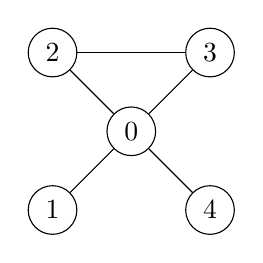
\begin{tikzpicture}
        \node[circle, draw] (0) at (1,1) {0};
        \node[circle, draw] (1) at (0,0) {1};
        \node[circle, draw] (2) at (0,2) {2};
        \node[circle, draw] (3) at (2,2) {3};
        \node[circle, draw] (4) at (2,0) {4};

        \draw (0) -- (4);
        \draw (0) -- (3);
        \draw (0) -- (2);
        \draw (0) -- (1);
        \draw (2) -- (3);
    \end{tikzpicture}

    In class, we used $k = 2$. In the following, you are being asked to illustrate the reductions for the same
    $G$ but other values of $k$.

    \begin{parts}
        \part[6]

        Show the {\em extended} incidence matrix for $G$ that incorporates Higher-Order Digits (HOD) and edge rows.
        In the last row, show the target $T$; assume $k = 1$

        \begin{tabular}{| l| c | c | c | c | c | c|} \hline
                      & $4^5$ & $4^4$     & $4^3$     & $4^2$     & $4^1$     & $4^0$     \\
                      & HOD1  & ~~$e_4$~~ & ~~$e_3$~~ & ~~$e_2$~~ & ~~$e_1$~~ & ~~$e_0$~~ \\ \hline
            $v_0$~~~~ & 1     & 0         & 1         & 1         & 1         & 1         \\ \hline
            $v_1$     & 1     & 0         & 1         & 0         & 0         & 0         \\ \hline
            $v_2$     & 1     & 1         & 0         & 1         & 0         & 0         \\ \hline
            $v_3$     & 1     & 1         & 0         & 0         & 1         & 0         \\ \hline
            $v_4$     & 1     & 0         & 0         & 0         & 0         & 1         \\ \hline
            $e_0$     & 0     & 0         & 0         & 0         & 0         & 1         \\ \hline
            $e_1$     & 0     & 0         & 0         & 0         & 1         & 0         \\ \hline
            $e_2$     & 0     & 0         & 0         & 1         & 0         & 0         \\ \hline
            $e_3$     & 0     & 0         & 1         & 0         & 0         & 0         \\ \hline
            $e_4$     & 0     & 1         & 0         & 0         & 0         & 0         \\ \hline \hline
            $T$       & 1     & 2         & 2         & 2         & 2         & 2         \\ \hline
        \end{tabular}

        \part[4] Either find a subset whose sum equals the target or argue that such a subset does not exist.

        There is no subset that sums to the target. Since $k=1$, only covering one vertex does not cover all edges.

        \part[6]

        Show the {\em extended} incidence matrix for $G$ that incorporates Higher-Order Digits (HOD) and edge rows.
        In the last row, show the target $T$; assume $k = 3$

        \begin{tabular}{| l| c | c | c | c | c | c|} \hline
                      & $4^5$ & $4^4$     & $4^3$     & $4^2$     & $4^1$     & $4^0$     \\
                      & HOD1  & ~~$e_4$~~ & ~~$e_3$~~ & ~~$e_2$~~ & ~~$e_1$~~ & ~~$e_0$~~ \\ \hline
            $v_0$~~~~ & 1     & 0         & 1         & 1         & 1         & 1         \\ \hline
            $v_1$     & 1     & 0         & 1         & 0         & 0         & 0         \\ \hline
            $v_2$     & 1     & 1         & 0         & 1         & 0         & 0         \\ \hline
            $v_3$     & 1     & 1         & 0         & 0         & 1         & 0         \\ \hline
            $v_4$     & 1     & 0         & 0         & 0         & 0         & 1         \\ \hline
            $e_0$     & 0     & 0         & 0         & 0         & 0         & 1         \\ \hline
            $e_1$     & 0     & 0         & 0         & 0         & 1         & 0         \\ \hline
            $e_2$     & 0     & 0         & 0         & 1         & 0         & 0         \\ \hline
            $e_3$     & 0     & 0         & 1         & 0         & 0         & 0         \\ \hline
            $e_4$     & 0     & 1         & 0         & 0         & 0         & 0         \\ \hline \hline
            $T$       & 3     & 2         & 2         & 2         & 2         & 2         \\ \hline
        \end{tabular}

        \part[4] Either find a subset whose sum equals the target or argue that such a subset does not exist.

        There is a subset that sums to the target. The subset is $\{v_0, v_1, v_2\}$.

    \end{parts}
    \clearpage

    \question[30] [W13, \stars{2}] In this problem, you will reduce multiple instances of the vertex cover problem to their corresponding CLIQUE instances. Assume that the inputs to VC are $\langle{G, k}\rangle$, the inputs to IS are $\langle{H, l}\rangle$, and the inputs to CLIQUE are $\langle{J, m}\rangle$.

    For all vertex cover instances, use the following graph, $G$:

    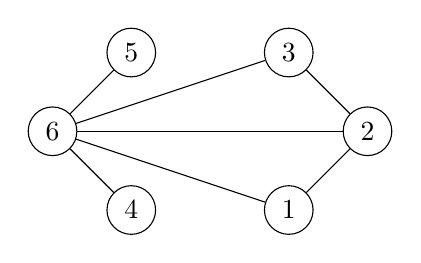
\begin{tikzpicture}
        \node[circle, draw] (1) at (2,0) {1};
        \node[circle, draw] (2) at (3,1) {2};
        \node[circle, draw] (3) at (2,2) {3};
        \node[circle, draw] (4) at (0,0) {4};
        \node[circle, draw] (5) at (0,2) {5};
        \node[circle, draw] (6) at (-1,1) {6};

        \draw (1) -- (2);
        \draw (1) -- (6);
        \draw (2) -- (3);
        \draw (2) -- (6);
        \draw (3) -- (6);
        \draw (4) -- (6);
        \draw (5) -- (6);
    \end{tikzpicture}

    \begin{parts}
        \part[5] For each of the following values of $k$, is there a vertex cover of size $k$ over $G$?

        \begin{itemize}
            \item $k=1$: $\square$ Yes $\blacksquare$ No
            \item $k=2$: $\blacksquare$ Yes $\square$ No
            \item $k=3$: $\blacksquare$ Yes $\square$ No
            \item $k=4$: $\blacksquare$ Yes $\square$ No
            \item $k=5$: $\blacksquare$ Yes $\square$ No
        \end{itemize}

        \part[5] Given the above graph $G$, draw the graph, $H$, that will be used as the input to the IS problem in order to solve this VC instance using IS.

        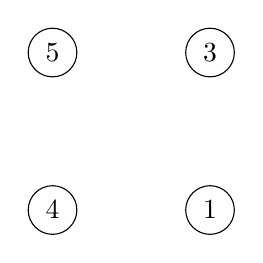
\begin{tikzpicture}
            \node[circle, draw] (1) at (2,0) {1};
            \node[circle, draw] (3) at (2,2) {3};
            \node[circle, draw] (4) at (0,0) {4};
            \node[circle, draw] (5) at (0,2) {5};
        \end{tikzpicture}

        \part[5] For each of the following values of $k$, what value of $l$ that will be used as the input to the IS problem in order to solve this VC instance using IS?

        \begin{itemize}
            \item $k=1$: $\boxed{\text{5}}$
            \item $k=2$: $\boxed{\text{4}}$
            \item $k=3$: $\boxed{\text{3}}$
            \item $k=4$: $\boxed{\text{2}}$
            \item $k=5$: $\boxed{\text{1}}$
        \end{itemize}

        \part[5] Given the graph $H$ you created in part (b), draw the graph, $J$, that will be used as the input to the CLIQUE problem in order to solve this IS instance using CLIQUE.

        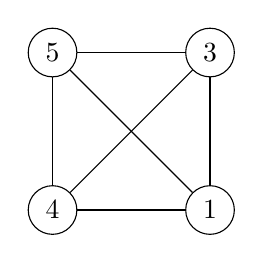
\begin{tikzpicture}
            \node[circle, draw] (1) at (2,0) {1};
            \node[circle, draw] (3) at (2,2) {3};
            \node[circle, draw] (4) at (0,0) {4};
            \node[circle, draw] (5) at (0,2) {5};

            \draw (5) -- (3);
            \draw (5) -- (1);
            \draw (5) -- (4);
            \draw (3) -- (4);
            \draw (1) -- (3);
            \draw (1) -- (4);
        \end{tikzpicture}

        \part[5] Given the following possible values of for $l$ from part (c), what value of $m$ will be used as the input to the CLIQUE problem in order to solve this IS instance using CLIQUE?

        \begin{itemize}
            \item $l=1$: $\boxed{\text{1}}$
            \item $l=2$: $\boxed{\text{2}}$
            \item $l=3$: $\boxed{\text{3}}$
            \item $l=4$: $\boxed{\text{4}}$
            \item $l=5$: $\boxed{\text{5}}$
        \end{itemize}

        \part[5] For the graph $J$ from part (d), and each of the following values of $m$ from part (e), is there a clique of size $m$ in $J$?

        \begin{itemize}
            \item $m=1$: $\blacksquare$ Yes $\square$ No
            \item $m=2$: $\blacksquare$ Yes $\square$ No
            \item $m=3$: $\blacksquare$ Yes $\square$ No
            \item $m=4$: $\blacksquare$ Yes $\square$ No
            \item $m=5$: $\square$ Yes $\blacksquare$ No
        \end{itemize}

    \end{parts}

    \textit{Once you have completed all parts of this question, make sure that your answers make sense. Are your answers for part (f) consistent with your answers in part (a)?}

    \clearpage

    \question[40][W14, \stars{5}]
    Consider the following problems:
    \begin{mdframed}
        \textbf{Subset Sum}

        Given a set of integers $U = \{u_1, u_2, u_3, \dots, u_n\}$ and a target sum $T$, the Subset Sum problem asks whether there exists a subset $S \subseteq U$ such that the sum of the elements in $S$ is equal to $T$.

        For example, consider the set $U = \{3, 34, 4, 12, 5, 2\}$ and a target sum $T = 9$. A possible solution is the subset $S = \{4, 5\}$, since the sum of the elements in $S$ is $4 + 5 = 9$, which equals the target sum $T$. The Subset Sum problem determines whether such a subset exists for a given set and target sum.
    \end{mdframed}

    \begin{mdframed}
        \textbf{Set Partition}

        Given a set of integers $U = \{u_1, u_2, u_3, \dots, u_n\}$, the Set Partition problem asks if it is possible to partition this set into two subsets $S_1$ and $S_2$ such that each element of $U$ is included in exactly one of the subsets and the sum of the elements in $S_1$ is equal to the sum of the elements in $S_2$.

        For example, consider the set $U = \{1, 2, 3, 4\}$. A possible partition meeting the criteria would be $S_1 = \{1, 4\}$ and $S_2 = \{2, 3\}$, since the sum of the elements in both subsets is 5, and every element of $U$ is present in either $S_1$ or $S_2$ exactly once. The Set Partition problem determines whether such a partition exists for a given set.
    \end{mdframed}

    Prove Set Partition (SP) is NP-Complete by reducing Subset Sum (SS) to Set Partition. %DO NOT reduce Set Partition to Subset Sum! This is simpler but does not prove Set Partition is NPC (and you will get a 0 on this problem if you do).

    \begin{parts}
        \part[5] Prove Set Partition is in NP (you shouldn't need more than a sentence or two).

        Set Partition is in NP because given a partition of the set, we can verify that the sum of the elements in each subset is equal.

        \part[10] Given the Subset Sum problem with a set $U$ and a target sum $T$, identify the single element that needs to be added to $U$ to transform it into a valid instance of the Set Partition problem. What is this element and how does it facilitate the reduction? (one paragraph).

        The element that needs to be added to $U$ is $2T$. This element facilitates the reduction because it ensures that the sum of the elements in $U$ is even. This is important because the Set Partition problem requires that the sum of the elements in each subset is equal. By adding $2T$, we ensure that the sum of the elements in $U$ is even, which is a necessary condition for a valid partition.

        \part[25] Provide a comprehensive argument for the correctness of your reduction from the SS problem to the SP problem.

        To prove Set Partition (SP) is NP-Complete, we need to establish its NP-membership and NP-hardness. We've already shown SP is in NP. To prove NP-hardness, we reduce Subset Sum (SS) to SP. Given an SS instance with set $U$ and target sum $T$, we add $2T$ to $U$ to ensure an even sum. If there's a subset $S \subseteq U$ with sum $T$, we partition $U$ into $S_1$ and $S_2$ with equal sums by adding $2T$. Conversely, if $U$ can be partitioned into $S_1$ and $S_2$ with equal sums, removing $2T$ yields a subset $S$ with sum $T$. Thus, SS reduces to SP, proving SP is NP-hard. Since SP is in NP and NP-hard, it's NP-Complete.






    \end{parts}

    % close the document
\end{questions}
\end{document}